\chapter{Evaluación Experimental}
\label{capitulo4}
\lhead{Capítulo 4. \emph{Evaluación Experimental}}

Este capítulo consiste en la descripción del diseño experimental empleado durante la evaluación de los métodos introducidos en los capítulos anteriores, así como el análisis de los resultados obtenidos de dicha evaluación. El objetivo de este estudio radica en la comparación empírica de cinco metaheurísticas (\emph{i.e.} GGA, SGA, CHC, PBIL y PSO) adaptadas para encontrar soluciones al problema de selección de instancias. Adicionalmente, se pretende estudiar el impacto de la aplicación de estrategias alternativas de generación de soluciones iniciales: disminuyendo la probabilidad de aparición de cada bit (de $50\%$ a $5\%$) y modificando dichas probabilidades en función de los subconjuntos de instancias generados por diferentes algoritmos heurísticos (\emph{i.e.} CNN, NEHS, Closest NE y Farthest NE).

\section{Diseño Experimental}

En este trabajo, el estudio experimental busca medir el impacto de 
\begin{inparaenum}[\itshape a\upshape)]
\item las metaheurísticas usadas y
\item las estrategias de inicialización aplicadas,
\end{inparaenum}
en los resultados obtenidos en términos de los objetivos del problema de SI y el tiempo de ejecución. Para esto se hace uso de varios conjuntos de datos, que ayuden a identificar los efectos de los diferentes factores a evaluar.
La metodología seguida debe permitir la generalización del comportamiento tanto de las metaheurísticas como de las estrategias de generación de soluciones iniciales, con la finalidad de comparar los resultados obtenidos y establecer los métodos más efectivos frente al problema de selección de instancias.

\subsection{Conjuntos de datos}
\label{data-section}

Un factor esencial en la evaluación de métodos de selección de instancias es el conjunto de datos utilizado; la distribución de los datos, el número de instancias y atributos, y la cantidad de datos ruidosos, son solo algunos de los elementos que modifican el espacio de búsqueda del problema y por ende la efectividad de los algoritmos heurísticos para encontrar buenas soluciones. Los conjuntos de datos usados en este trabajo pertenecen al \emph{UCI Machine Learning Repository} \cite{BacheLichman:2013} y al \emph{KEEL Data-Mining Software Tool} \cite{alcala2010keel}.

Los 14 conjuntos seleccionados fueron separados en 3 grupos en función del número de instancias de cada conjunto. En la tabla \ref{data-small} se presentan 9 conjuntos con menor cantidad de instancias (menor a 1000).

\begin{table}[h!]
\centering
\begin{tabular}{l c c c}
\hline
\textsc{Conjunto} & \textsc{Instancias} & \textsc{Atributos} & \textsc{Clases} \\
\hline
\hline
Cleveland & 297 & 13 &  5 \\
Glass     & 214 &  9 &  7 \\
Iris      & 150 &  4 &  3 \\
Led7Digit & 500 &  7 & 10 \\
Monk      & 432 &  6 &  2 \\
Pima      & 768 &  8 &  2 \\
WDBC      & 569 & 30 &  2 \\
Wine      & 178 & 13 &  3 \\
Wisconsin & 683 &  9 &  2 \\
\hline
\end{tabular}
\caption{Conjuntos de datos pequeños}
\label{data-small}
\end{table}

En la tabla \ref{data-med} se describen dos conjuntos de datos caracterizados como de tamaño medio. Estos conjuntos se caracterizan por tener un número de instancias entre 1000 y 6000.

\begin{table}[h!]
\centering
\begin{tabular}{l c c c}
\hline
\textsc{Conjunto} & \textsc{Instancias} & \textsc{Atributos} & \textsc{Clases} \\
\hline
\hline
Banana       &  5300 &  2 &  2 \\
Segmentation &  2100 & 19 &  7 \\
\hline
\end{tabular}
\caption{Conjuntos de datos medianos}
\label{data-med}
\end{table}

Finalmente, los 3 conjuntos con mayor número de instancias se presentan en la tabla \ref{data-big}. Estos conjuntos contienen un número de instancias mayor a 6000 junto con un número de atributos alto.

\begin{table}[h!]
\centering
\begin{tabular}{l c c c}
\hline
\textsc{Conjunto} & \textsc{Instancias} & \textsc{Atributos} & \textsc{Clases} \\
\hline
\hline
Penbased    & 10992 & 16 & 10 \\
Satimage    &  6435 & 36 &  6 \\
Thyroid     &  7200 & 21 &  3 \\
\hline
\end{tabular}
\caption{Conjuntos de datos grandes}
\label{data-big}
\end{table}

\subsection{Particiones y ejecuciones}

Los conjuntos de datos considerados en la sección anterior son particionados usando la estrategia de validación cruzada en 10 grupos (10-\emph{fold cross-validation}). El conjunto inicial de instancias $T$ es dividido en 10 subconjuntos disjuntos de igual tamaño $T_1, T_2, \dots T_{10}$. Cada conjunto $T_i$ mantiene la proporción de distribución de las clases del conjunto original $T$. En función de esta partición, se definen los pares de conjuntos $(T'_i, T_i)$, con $i = 1 \dots 10$, donde $T'_i = T \setminus T_i$.

El conjunto $T'_i$, también conocido como el conjunto de ``entrenamiento'', es usado por las metaheurísticas durante el proceso de búsqueda para evaluar soluciones intermedias, en vez de usar $T$. %, se usa el conjunto $T'_i$ como el conjunto de instancias inicial.
Las instancias restantes (pertenecientes al conjunto $T_i$) son usadas como conjunto de ``validación'', \emph{i.e.} la mejor solución encontrada durante la ejecución, es usada para clasificar las instancias desconocidas de $T_i$.

En base a esta estrategia, se definen los criterios de comparación empleados en el presente trabajo. Dada una solución $R \subseteq T'_i$ al problema de SI encontrada por una metaheurística, se considera:

\begin{itemize}
\item \emph{Error de Entrenamiento}\\
El porcentaje de instancias en $T'_i$ mal clasificadas usando $R$ como conjunto de prototipos en un clasificador 1-NN. Para el cálculo de esta métrica no se remueven las instancias antes de ser clasificadas (\emph{Leave-one-out cross-validation}), por lo que toda instancia en $R$ se considera correctamente clasificada.
\item \emph{Error de Validación}\\
El porcentaje de instancias en $T_i$ mal clasificadas usando $R$ como conjunto de prototipos en un clasificador 1-NN.
\item \emph{Tamaño}\\
El tamaño de $R$ en función de $T'_i$ (\emph{i.e.} $\frac{100 \vert R \vert}{\vert T'_i \vert}$).
\item \emph{Tiempo}\\
Segundos empleados por el algoritmo durante la búsqueda.
\end{itemize} 

Cada metaheurística es evaluada usando los 10 pares de conjuntos $(T'_i, T_i)$. Por cada par de conjunto entrenamiento-validación se realizan 3 repeticiones. \emph{i.e.} un total de 30 ejecuciones de una metaheurística para un conjunto de datos y un tipo de inicialización particular. Las ejecuciones fueron realizadas de manera independiente en máquinas de tipo \texttt{c3.2xlarge} de \emph{Amazon EC2}, que disponen de 8 CPUs Intel Xeon E5-2680 v2 (Ivy Bridge), 15GB de memoria RAM y 80GB de disco duro de estado sólido.

Todos los experimentos se realizaron bajo el sistema operativo Amazon Linux AMI 2014.03.2 y utilizando GCC 4.8.2. En este sentido, la implementación realizada aprovecha la arquitectura usada durante la implementación, evaluando las soluciones intermedias mediante la creación de hilos.

\subsection{Parámetros}
\label{sec-parametros}

Cada metaheurística depende de un conjunto de parámetros que regulan el proceso de búsqueda sobre el espacio de posibles soluciones. El valor de cada parámetro y la interacción entre ellos, determinan el comportamiento del algoritmo y su capacidad para encontrar buenas soluciones. Sin embargo, los valores que indican el buen comportamiento de una metaheurística, son altamente dependientes del problema en general, e incluso de la instancia particular que se pretenda evaluar. Esto lo convierte en un proceso complejo, que a menudo conlleva a un diseño factorial con el fin de estudiar la influencia de los parámetros y sus interacciones en asegurar la calidad de las soluciones obtenidas.

En el presente trabajo se realizó la entonación de las metaheurísticas seleccionadas en los capítulos anteriores. Los resultados obtenidos de este proceso se describen en el Apéndice \ref{apendiceA}. En la tabla \ref{table-parameters} se presentan los parámetros seleccionados para cada metaheurística.

\begin{table}[h!]
\centering
\begin{tabular}{l c c c c c}
\hline
\multirow{2}{*}{\textsc{Parámetros}}
	& \multicolumn{5}{c}{\textsc{Algoritmos}} \\\cline{2-6}
	& GGA & SGA & CHC & PBIL & PSO \\
\hline
\hline
Iteraciones        &  1000 &  1000 &  1000 &  1000 &  1000 \\
Población          &    50 &    30 &    30 &    40 &     5 \\
Prob. de Cruce     &   0.9 &   1.0 &     - &     - &     - \\
Prob. de Mutación  & 0.001 & 0.001 &     - & 0.001 &     - \\
Mutation Shift     &     - &     - &     - &  0.01 &     - \\
Learning Rate      &     - &     - &     - &   0.1 &     - \\
Neg. Learning Rate &     - &     - &     - &  0.01 &     - \\
Partículas         &     - &     - &     - &     - &     5 \\
Velocidad Máxima   &     - &     - &     - &     - &   0.2 \\
Inercia            &     - &     - &     - &     - &   0.9 \\
c1                 &     - &     - &     - &     - &   0.1 \\
c2                 &     - &     - &     - &     - &   0.1 \\
\hline
\end{tabular}
\caption{Parámetros usados en cada metaheurística}
\label{table-parameters}
\end{table}

\subsection{Tablas de resultados}

En la sección \ref{sec-res} son presentados y analizados los resultados obtenidos del proceso experimental. Las tablas de resultados deben permitir identificar las mejores estrategias de inicialización o las mejores metaheurísticas, según corresponda.

En primer lugar, se presenta una tabla con los resultados promedio de cada metaheurística, en función de los 4 criterios de comparación descritos en la subsección \ref{sec-parametros}. Para una metaheurística particular, se promedian sus resultados para los conjuntos de datos que correspondan.

Sin embargo, al promediar los resultados puede perderse información relevante, puesto que el comportamiento de una metaheurística depende del conjunto de datos que se use para evaluarla. Por esta razón, se introducen las tablas de ranking, que presentan información adicional que permite comparar las metaheurísticas bajo un mismo contexto. Por cada conjunto de datos, las metaheurísticas son rankeadas de acuerdo a sus resultados en una métrica particular. A partir del ordenamiento en cada conjunto de datos, la tabla muestra el ranking promedio de cada metaheurística y el número de veces que logró el mejor resultado. Estos valores son calculados usando las métricas de tamaño, error de validación y la combinación lineal de ambos.

Ambas tablas son usadas para presentar los resultados por cada estrategia de inicialización. Para la primera tabla, se promedian los resultados no solo por conjunto de datos, sino también por metaheurística. Para las tablas de ranking ocurre lo mismo: los ordenamientos son realizados por cada combinación de metaheurística y conjunto de datos evaluados.

\section{Resultados}
\label{sec-res}

En esta sección se presentan los resultados obtenidos durante la evaluación experimental. En la sección \ref{sec-comp-inits} se comparan diferentes estrategias de inicialización de soluciones con representación binaria,
\begin{inparaenum}[\itshape a\upshape)]
\item evaluando el impacto de disminuir la probabilidad de aparición de bits, y
\item modificando dicha probabilidad de forma individual a lo largo de la cadena de bits, de un valor constante $\delta$ para todos los bits, a valores que favorezcan a las instancias pertenecientes a los conjuntos seleccionados por algoritmos heurísticos al problema de SI.
\end{inparaenum}
Una vez seleccionada la mejor estrategia de inicialización, en la sección \ref{sec-comp-meta} se comparan los resultados obtenidos por las 5 metaheurísticas descritas. Se concluye con un estudio que busca determinar (en caso que existan) aquellas metaheurísticas que se comporten consistentemente mejor que el resto.

\subsection{Comparación entre inicializaciones}
\label{sec-comp-inits}

Bajo el contexto del problema de SI, modificar la estrategia de inicialización de soluciones tiene un objetivo claro: iniciar el proceso de búsqueda en ``buenas'' soluciones. Una buena solución al problema de SI debe minimizar tanto la cardinalidad del conjunto $R$, como el error de clasificación usando $R$ como conjunto de prototipos. En este sentido, se propone disminuir la probabilidad de aparición de bits $\delta$ para reducir la cardinalidad de soluciones iniciales, y modificar la probabilidad de cada bit de forma individual, beneficiando a instancias seleccionadas por diferentes algoritmos heurísticos, con la intensión de reducir el error de clasificación.

Con la finalidad de comparar diferentes estrategias de inicialización, se realizaron experimentos sobre los conjuntos de datos grandes (Tabla \ref{data-big}). Los resultados obtenidos son presentados y analizados a continuación.

\subsubsection{Inicialización disminuyendo la probabilidad de aparición de bit}

Con la finalidad de reducir la cardinalidad de las soluciones iniciales generadas, en un intento de reducir el número de iteraciones necesarias para conseguir porcentajes de reducción aceptables, este estudio propone la reducción de la probabilidad de aparición de bits $\delta$. En esta sección se estudia el impacto de la disminución propuesta, usando 3 posibles valores: $50\%$, $25\%$ y $5\%$.

En la tabla \ref{table-unif} se presentan los resultados promedio de la evaluación de las 5 metaheurísticas sobre los conjuntos de datos grandes, modificando únicamente el parámetro $\delta$ (probabilidad de aparición de bit).

\begin{table}[h!]
\centering
\begin{tabular}{c c c c c}
\hline
\multirow{2}{*}{$\delta$}
	& \multirow{2}{*}{\textsc{Tiempo}}
	& \multirow{2}{*}{\textsc{Tamaño}}
	& \multicolumn{2}{c}{$\%$ de \textsc{Error}} \\\cline{4-5}
 & & & \scriptsize{Entrenamiento} & \scriptsize{Validación} \\
\hline
\hline
$50\%$ & 1324.96 & 37.09 & \textbf{2.94} & \textbf{6.60} \\
$25\%$ & 1193.26 & 19.83 & 4.14 & 6.71 \\
$5\%$  & \textbf{893.24} & \textbf{4.67} & 6.25 & 7.28 \\
\hline
\end{tabular}
\caption[Resultados al disminuir la probabilidad de aparición de bit $\delta$]{Resultados promedio de las 5 metaheurísticas\\frente a los conjuntos de datos grandes, usando una\\probabilidad de aparición de bit $\delta$ igual a $50\%$, $25\%$ y $5\%$.}
\label{table-unif}
\end{table}

Estos datos corroboran la hipótesis de que al usar $\delta = 50\%$, es necesario un mayor número de iteraciones para converger a soluciones con porcentajes de reducción aceptables \cite{cano2003using}. Como era de esperarse, la disminución del parámetro $\delta$ implica una reducción similar en términos del tamaño de las soluciones encontradas. Esto a su vez, supone una disminución importante en el tiempo de ejecución de los algoritmos, debido a que la evaluación de soluciones intermedias depende en gran medida de la cardinalidad de dichas soluciones.

\begin{figure}[h!]
\centering
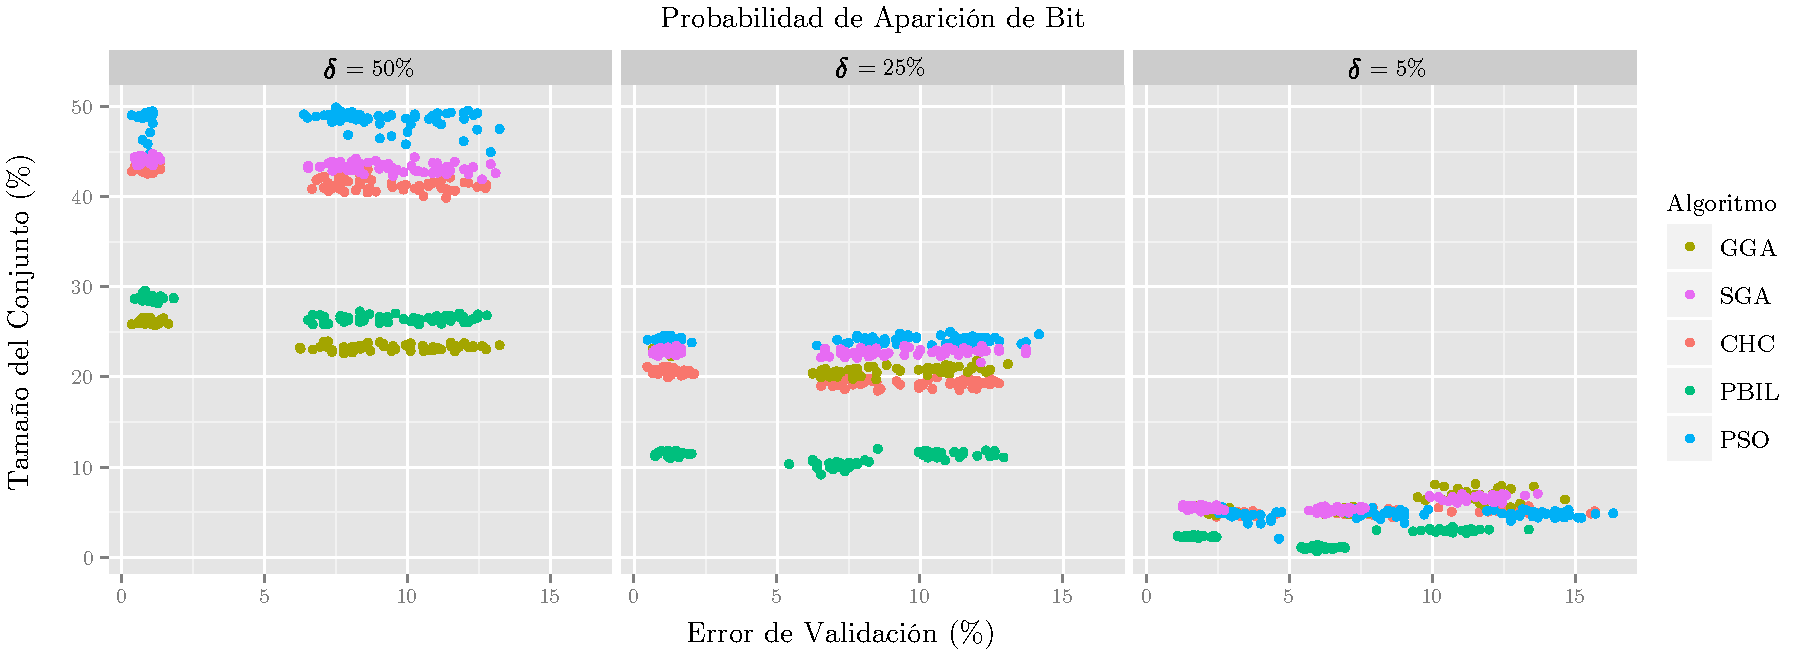
\includegraphics[width=\textwidth]{uniforme.pdf}
\caption[Tamaño \emph{vs} error de validación modificando $\delta$]{Tamaño del conjunto \emph{vs} error de validación en\\ejecuciones de las metaheurísticas usando $\delta$ igual a $50\%$, $25\%$ y $5\%$.}
\label{fig-unif}
\end{figure}

En la figura \ref{fig-unif} resultan evidentes las diferencias en el tamaño de las soluciones encontradas usando las 3 probabilidades seleccionadas. No es únicamente una diferencia promedio: la inicialización usando $\delta = 5\%$ logra que las 5 metaheurísticas consigan soluciones más consistentes en términos de reducción.

Sin embargo, la disminución del parámetro $\delta$ conlleva a un aumento en los errores de entrenamiento y validación. No obstante, en ambos casos los errores se mantienen en valores aceptables, y en el caso del error de validación, la diferencia es poco significativa.

\begin{table}[h!]
\centering
\begin{tabular}{c c c|c c c|c c c}
\hline
\multicolumn{3}{c|}{\textsc{Error de Validación}}
	& \multicolumn{3}{c|}{\textsc{Tamaño}}
	& \multicolumn{3}{c}{\textsc{Error + Tamaño}} \\
\hline
$\delta$ & Rank & Mejor & $\delta$ & Rank & Mejor & $\delta$ & Rank & Mejor \\
\hline
\hline
$50\%$ & 1.73 & 9 & $5\%$  & 1.0 & 15 & $5\%$  & 1.0 & 15 \\
$25\%$ & 1.93 & 4 & $25\%$ & 2.0 &  0 & $25\%$ & 2.0 &  0 \\
$5\%$  & 2.33 & 2 & $50\%$ & 3.0 &  0 & $50\%$ & 3.0 &  0 \\
\hline
\end{tabular}
\caption[Ranking de valores probabilidad de aparición de bit $\delta$]{Ranking de probabilidades $\delta$ según el tamaño y error de validación, considerando los promedios de las ejecuciones de cada algoritmo frente a los conjuntos de datos grandes. Por cada valor de $\delta$, se presenta su ranking promedio (\emph{Rank}) y el número de veces que obtuvo los mejores resultados (\emph{Mejor}).}
\label{table-unif-rank}
\end{table}

A pesar de que las diferencias en el error de validación favorecen el uso de\linebreak$\delta = 50\%$, la disminución de la probabilidad de aparición de bit al $5\%$ supone beneficios importantes en relación a la reducción alcanzada (ver la tabla \ref{table-unif-rank}) y al tiempo de ejecución. Por esta razón, se decidió usar $\delta = 5\%$ durante el resto de la evaluación experimental.

\subsubsection{Inicialización usando algoritmos heurísticos}

En esta sección se evalúa el impacto de generar soluciones iniciales, modificando de forma independiente la probabilidad de aparición de bits lo largo la cadena que representa una solución al problema de SI. El enfoque estándar asigna un valor de probabilidad constante igual a $\delta$, \emph{i.e.} todos los bits tienen igual probabilidad de estar ``prendidos''. En el presente trabajo, se propone una técnica de modificación que asigna valores de probabilidad diferente en base a la selección realizada por algoritmos heurísticos.

\begin{table}[h!]
\centering
\begin{tabular}{l c c c c}
\hline
\multirow{2}{*}{\textsc{Inicialización}}
	& \multirow{2}{*}{\textsc{Tiempo}}
	& \multirow{2}{*}{\textsc{Tamaño}}
	& \multicolumn{2}{c}{$\%$ de \textsc{Error}} \\\cline{4-5}
 & & & \scriptsize{Entrenamiento} & \scriptsize{Validación} \\
\hline
\hline
Constante  & \textbf{893.24} & \textbf{4.67} & 6.25 & \textbf{7.28} \\
NEHS       & 958.94 & 4.70 & \textbf{6.20} & \textbf{7.28} \\
CNN        & 921.68 & 5.11 & 6.27 & 7.85 \\
FarthestNE & 932.19 & 4.98 & 6.94 & 7.67 \\
ClosestNE  & 932.75 & 5.56 & 7.21 & 8.95 \\
\hline
\end{tabular}
\caption[Resultados usando probabilidades constantes y basadas en heurísticas]{Resultados promedio de las 5 metaheurísticas frente a los\\conjuntos de datos grandes, usando valores de probabilidad constante\\y basados en algoritmos heurísticos.}
\label{table-inits}
\end{table}

En la tabla \ref{table-inits} se presentan los resultados promedio de las 5 metaheurísticas descritas, generando soluciones iniciales con un valor de probabilidad constante o con valores en función de las selecciones generadas por CNN, NEHS, Closest NE y Farthest NE. Los datos en tiempo de ejecución son previsibles, debido al tiempo que requieren estos algoritmos heurísticos para generar sus soluciones. Sin embargo, contrario a lo esperado, estas modificaciones no mejoran significativamente los porcentajes de error obtenidos mediante el uso de una probabilidad constante. Más aún, las soluciones basadas en CNN, Closest NE y Farthest NE empeoran los resultados en todos los aspectos. Solo probabilidades en función de NEHS reportan resultados alentadores, mejorando el error de entrenamiento e igualando el error de validación frente al uso de una probabilidad constante.

La figura \ref{fig-inits} confirma los aspectos señalados: el comportamiento de inicializaciones basadas en CNN, Closest NE y Farthest NE difieren significativamente del comportamiento de aquellas basadas en NEHS o con probabilidad constante. Estas últimas muestran un comportamiento similar en función de ambos objetivos del problema.

\begin{figure}[h!]
\centering
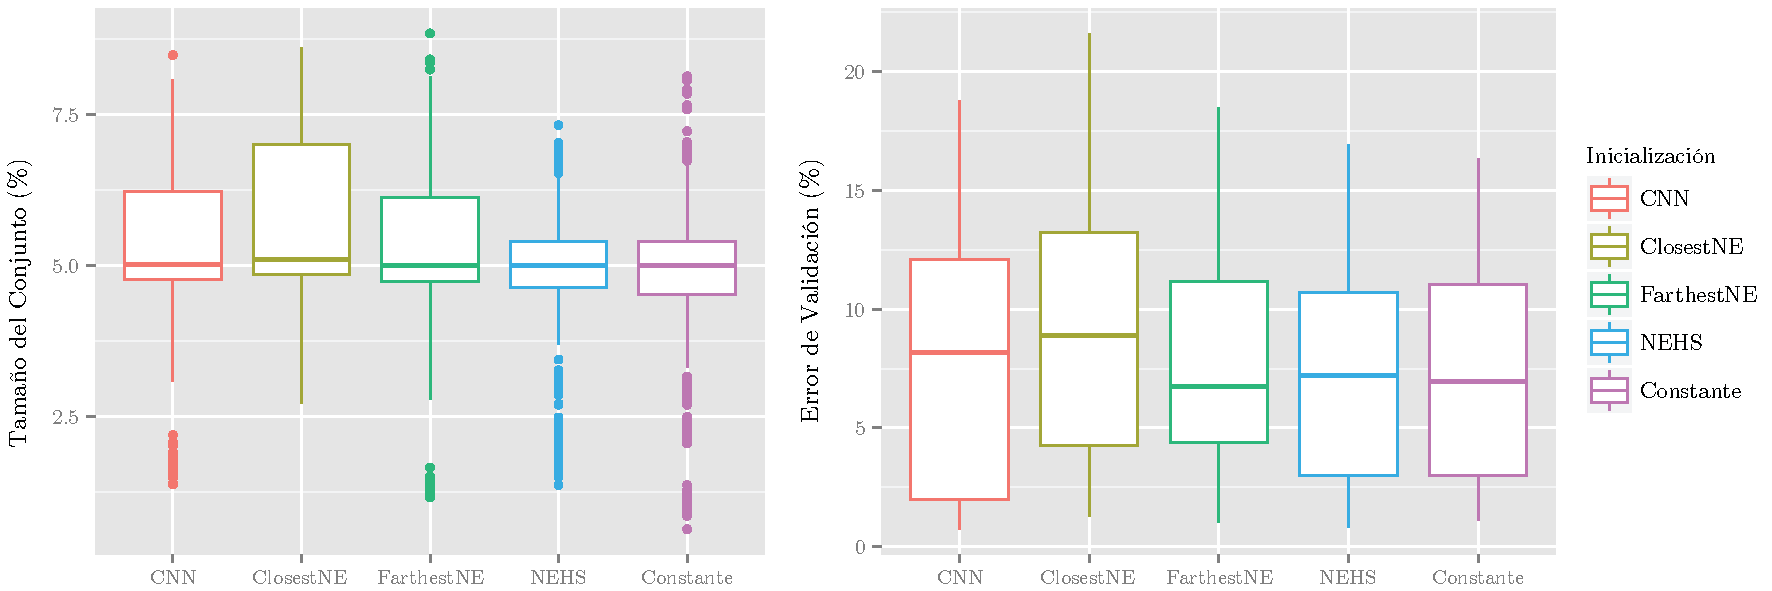
\includegraphics[width=\textwidth]{inits-boxplot.pdf}
\caption[Tamaño y error de validación usando algoritmos heurísticos]{Diagramas de caja del tamaño y error de validación usando\\valores de probabilidad constante y basados en algoritmos heurísticos.}
\label{fig-inits}
\end{figure}

Sin embargo, la tabla \ref{table-inits-rank} sugiere que una inicialización basada en NEHS resulta conveniente en función de los dos objetivos del problema, siendo el que presenta mejor ranking promedio en base al error de validación y a la combinación lineal entre el error y el tamaño del conjunto seleccionado. En función de estos resultados, se usa NEHS como heurística de inicialización de las ejecuciones realizadas en la sección \ref{sec-comp-meta}, cuya finalidad es determinar aquellas metaheurísticas que se comporten consistentemente mejor que las demás.

\begin{table}[h!]
\centering
\begin{tabular}{l c c|l c c|l c c}
\hline
\multicolumn{3}{c|}{\textsc{Error de Validación}}
	& \multicolumn{3}{c|}{\textsc{Tamaño}}
	& \multicolumn{3}{c}{\textsc{Error + Tamaño}} \\
\hline
Inicialización & Rank & Mejor & Inicialización & Rank & Mejor & Inicialización & Rank & Mejor \\
\hline
\hline
NEHS       & 2.06 & 4 & Constante  & 1.86 & 6 & NEHS       & 2.00 & 5 \\
Constante  & 2.40 & 2 & NEHS       & 2.26 & 3 & Constante  & 2.20 & 2 \\
CNN        & 2.86 & 4 & FarthestNE & 2.86 & 4 & CNN        & 2.93 & 4 \\
FarthestNE & 2.93 & 5 & CNN        & 3.60 & 2 & FarthestNE & 3.06 & 4 \\
ClosestNE  & 4.73 & 0 & ClosestNE  & 4.40 & 0 & ClosestNE  & 4.80 & 0 \\
\hline
\end{tabular}
\caption[Ranking de probabilidades constantes o basadas en heurísticas]{Ranking de inicializaciones con probabilidades constantes o basadas en heurísticas, según el tamaño y error de validación, considerando los promedios de las ejecuciones de cada algoritmo frente a los conjuntos de datos grandes. Por cada inicialización, se presenta su ranking promedio (\emph{Rank}) y el número de veces que obtuvo los mejores resultados (\emph{Mejor}).}
\label{table-inits-rank}
\end{table} 

\subsection{Comparación entre metaheurísticas}
\label{sec-comp-meta}

Para controlar el proceso de búsqueda, cada metaheurística emplea técnicas diversas para recorrer el espacio de posibles soluciones. Su capacidad para encontrar buenas soluciones está íntimamente ligado al problema que se desea resolver, la representación de sus soluciones, la función de objetivo, entre otros factores. La distribución del espacio de búsqueda puede alterar significativamente la efectividad de una metaheurística particular. Por esta razón, al estudiar el comportamiento de diferentes metaheurísticas frente al problema de SI, es necesario identificar aquellas metaheurísticas que exhiban mejor capacidad para seleccionar subconjuntos de instancias que cumplan con los objetivos planteados por el problema.

A continuación se presenta un estudio fraccionado del comportamiento de las 5 metaheurísticas, adaptadas en función de los resultados descritos en la sección \ref{sec-comp-inits}. Se describen los resultados obtenidos usando los conjuntos de datos caracterizados como pequeños, medianos y grandes. Finalmente, se realiza un análisis estadístico conjunto, con la finalidad de determinar si existen diferencias significativas entre las metaheurísticas.

\subsubsection{Resultados para conjuntos de datos pequeños}

En la tabla \ref{res-small} se presentan los resultados promedio de cada metaheurística, al ser evaluadas usando los conjuntos de datos pequeños. En función del error de clasificación en los conjuntos de entrenamiento y validación, GGA muestra mejores resultados que el resto de las metaheurísticas. Sin embargo, el error de validación alcanzado por las demás metaheurísticas, en particular los resultados de SGA y PBIL, son bastante cercanos. En términos de la reducción lograda, son PBIL y CHC los que seleccionan conjuntos de datos de menor tamaño, mientras que PSO es el que consigue los peores resultados.

Las mayores diferencias se ven reflejadas en los tiempos de ejecución, donde PSO y GGA requieren de un mayor número de segundos para concluir la búsqueda. No obstante, cabe destacar que sobre los conjuntos de datos pequeños, los tiempos de ejecución de estas metaheurísticas no son prohibitivos.

\begin{table}[h!]
\centering
\begin{tabular}{l c c c c}
\hline
\multirow{2}{*}{\textsc{Algoritmo}}
	& \multirow{2}{*}{\textsc{Tiempo}}
	& \multirow{2}{*}{\textsc{Tamaño}}
	& \multicolumn{2}{c}{$\%$ de \textsc{Error}} \\\cline{4-5}
 & & & \scriptsize{Entrenamiento} & \scriptsize{Validación} \\
\hline
\hline
GGA  &  5.51 & 4.66 & \textbf{10.94} & \textbf{17.89} \\
SGA  & \textbf{0.70} & 4.85 & 13.23 & 18.94 \\
CHC  &  1.75 & 3.44 & 14.15 & 19.45 \\
PBIL &  2.95 & \textbf{3.36} & 13.32 & 18.64 \\
PSO  & 10.59 & 6.28 & 18.64 & 21.90 \\
\hline
\end{tabular}
\caption[Resultados de metaheurísticas usando conjuntos de datos pequeños]{Resultados promedio de los conjuntos de\\datos pequeños, usando las metaheurísticas descritas.}
\label{res-small}
\end{table}

La tabla de rankings (Tabla \ref{res-small-rank}) ofrece otra perspectiva. PBIL domina los rankings en función del error de validación, el tamaño del conjunto seleccionado y la combinación de ambos objetivos. El ranking promedio de GGA y CHC en términos del error y el tamaño respectivamente, corroboran los resultados descritos anteriormente.

\begin{table}[h!]
\centering
\begin{tabular}{l c c|l c c|l c c}
\hline
\multicolumn{3}{c|}{\textsc{Error de Validación}}
	& \multicolumn{3}{c|}{\textsc{Tamaño}}
	& \multicolumn{3}{c}{\textsc{Error + Tamaño}} \\
\hline
Algoritmo & Rank & Mejor & Algoritmo & Rank & Mejor & Algoritmo & Rank & Mejor \\
\hline
\hline
PBIL & 2.00 & 4 & PBIL & 1.44 & 5 & PBIL & 1.55 & 6 \\
GGA  & 2.22 & 4 & CHC  & 1.88 & 3 & GGA  & 2.44 & 2 \\
SGA  & 2.66 & 1 & GGA  & 3.11 & 1 & CHC  & 2.88 & 0 \\
CHC  & 3.77 & 0 & SGA  & 3.88 & 0 & SGA  & 3.22 & 1 \\
PSO  & 4.33 & 0 & PSO  & 4.66 & 0 & PSO  & 4.88 & 0 \\
\hline
\end{tabular}
\caption[Ranking de metaheurísticas usando conjuntos de datos pequeños]{Ranking de metaheurísticas según el tamaño y error de validación, considerando los promedios de las ejecuciones de cada algoritmo frente a los conjuntos de datos pequeños. Por cada algoritmo, se presenta su ranking promedio (\emph{Rank}) y el número de veces que obtuvo los mejores resultados (\emph{Mejor}).}
\label{res-small-rank}
\end{table}

Los datos sugieren que PBIL representa la mejor alternativa para encontrar soluciones a instancias ``pequeñas'' del problema de SI, ya que logra buenos resultados tanto en términos de precisión de clasificación, como en términos de reducción. Sin embargo, GGA y CHC presentan resultados comparables, por lo que no deben descartarse.

\subsubsection{Resultados para conjuntos de datos medianos}

En la tabla \ref{res-med} se presentan los resultados obtenidos al evaluar las metaheurísticas frente a los conjuntos de datos medianos. Los tiempos de ejecución aumentan notablemente, y las diferencias en tiempo entre los diferentes algoritmos se mantienen: PSO y GGA requieren en promedio más del doble del tiempo que PBIL, y pueden tardar hasta 9 veces más que SGA y CHC. De nuevo, PBIL y GGA logran los mejores resultados en función del error de clasificación. Sin embargo, los porcentajes de error reportados (sobretodo en el conjunto de validación) no varían considerablemente entre metaheurísticas; a excepción de PSO, que exhibe los mayores errores de clasificación en ambos casos. Por último, el tamaño de los conjuntos encontrados por PBIL es menor que en el resto de algoritmos, aunque CHC también reporta una reducción considerable.

\begin{table}[h!]
\centering
\begin{tabular}{l c c c c}
\hline
\multirow{2}{*}{\textsc{Algoritmo}}
	& \multirow{2}{*}{\textsc{Tiempo}}
	& \multirow{2}{*}{\textsc{Tamaño}}
	& \multicolumn{2}{c}{$\%$ de \textsc{Error}} \\\cline{4-5}
 & & & \scriptsize{Entrenamiento} & \scriptsize{Validación} \\
\hline
\hline
GGA  & 80.49 & 6.02 &  \textbf{5.96} &  8.58 \\
SGA  & \textbf{8.67} & 5.80 &  6.76 &  8.92 \\
CHC  &  8.89 & 4.46 &  7.51 &  8.90 \\
PBIL & 38.06 & \textbf{2.72} &  6.06 &  \textbf{8.35} \\
PSO  & 97.98 & 5.55 & 10.66 & 11.83 \\
\hline
\end{tabular}
\caption[Resultados de metaheurísticas usando conjuntos de datos medianos]{Resultados promedio de los conjuntos de\\datos medianos, usando las metaheurísticas descritas.}
\label{res-med}
\end{table}

Estas observaciones son ratificadas con los datos de la tabla \ref{res-med-rank}, que muestra el dominio de los resultados dados por PBIL bajo las métricas del tamaño del conjunto seleccionado y el error de validación alcanzado. No obstante, los resultados reportados por CHC son interesantes en función del ranking conjunto, tomando en cuenta la diferencia en tiempo de ejecución existente en comparación con PBIL.

\begin{table}[h!]
\centering
\begin{tabular}{l c c|l c c|l c c}
\hline
\multicolumn{3}{c|}{\textsc{Error de Validación}}
	& \multicolumn{3}{c|}{\textsc{Tamaño}}
	& \multicolumn{3}{c}{\textsc{Error + Tamaño}} \\
\hline
Algoritmo & Rank & Mejor & Algoritmo & Rank & Mejor & Algoritmo & Rank & Mejor \\
\hline
\hline
PBIL & 1.5 & 1 & PBIL & 1.0 & 2 & PBIL & 1.0 & 2 \\
GGA  & 2.5 & 1 & CHC  & 2.0 & 0 & CHC  & 2.0 & 0 \\
SGA  & 3.0 & 0 & PSO  & 3.0 & 0 & GGA  & 3.5 & 0 \\
CHC  & 3.0 & 0 & GGA  & 4.5 & 0 & SGA  & 3.5 & 0 \\
PSO  & 5.0 & 0 & SGA  & 4.5 & 0 & PSO  & 5.0 & 0 \\
\hline
\end{tabular}
\caption[Ranking de metaheurísticas usando conjuntos de datos medianos]{Ranking de metaheurísticas según el tamaño y error de validación, considerando los promedios de las ejecuciones de cada algoritmo frente a los conjuntos de datos medianos. Por cada algoritmo, se presenta su ranking promedio (\emph{Rank}) y el número de veces que obtuvo los mejores resultados (\emph{Mejor}).}
\label{res-med-rank}
\end{table}

\subsubsection{Resultados para conjuntos de datos grandes}

Los resultados de las ejecuciones usando los conjuntos de datos grandes se presentan en la tabla \ref{res-big}. El tiempo requerido por las metaheurísticas para solucionar los conjuntos grandes es notablemente mayor que el requerido para conjuntos medianos. Esto es una consecuencia directa del aumento, no solo en el número de instancias, sino en el número de atributos de los datos: el fenómeno conocido como la \guillemotleft\emph{maldición de la dimensionalidad}\guillemotright. Son aumentos en el orden de 24, 22, 17, 12 y 2 veces el tiempo requerido por GGA, PSO, SGA, PBIL y CHC respectivamente, en comparación con los tiempos reportados para los conjuntos medianos.

\begin{table}[h!]
\centering
\begin{tabular}{l c c c c}
\hline
\multirow{2}{*}{\textsc{Algoritmo}}
	& \multirow{2}{*}{\textsc{Tiempo}}
	& \multirow{2}{*}{\textsc{Tamaño}}
	& \multicolumn{2}{c}{$\%$ de \textsc{Error}} \\\cline{4-5}
 & & & \scriptsize{Entrenamiento} & \scriptsize{Validación} \\
\hline
\hline
GGA  & 1938.78 & 5.58 & 6.11 & 7.13 \\
SGA  &  152.71 & 5.74 & 5.42 & 6.56 \\
CHC  & \textbf{22.37} & 5.00 & 7.35 & 8.08 \\
PBIL &  472.63 & \textbf{2.36} & \textbf{4.35} & \textbf{6.19} \\
PSO  & 2208.22 & 4.80 & 7.76 & 8.43 \\
\hline
\end{tabular}
\caption[Resultados de metaheurísticas usando conjuntos de datos grandes]{Resultados promedio de los conjuntos de\\datos grandes, usando las metaheurísticas descritas.}
\label{res-big}
\end{table}

En función del tamaño de los conjuntos seleccionados, los resultados de PBIL dominan los del resto de las metaheurísticas. Adicionalmente, los mejores resultados en términos del error de clasificación (ambos) son reportados por PBIL, conclusión respaldada por la tabla de rankings \ref{res-big-rank}. Sin embargo, los porcentajes de error logrados por SGA y GGA son competitivos frente a PBIL, lo cual se ve reflejado en los rankings promedio del error de validación y el ranking conjunto.

\begin{table}[h!]
\centering
\begin{tabular}{l c c|l c c|l c c}
\hline
\multicolumn{3}{c|}{\textsc{Error de Validación}}
	& \multicolumn{3}{c|}{\textsc{Tamaño}}
	& \multicolumn{3}{c}{\textsc{Error + Tamaño}} \\
\hline
Algoritmo & Rank & Mejor & Algoritmo & Rank & Mejor & Algoritmo & Rank & Mejor \\
\hline
\hline
PBIL & 1.00 & 3 & PBIL & 1.00 & 3 & PBIL & 1.00 & 3 \\
SGA  & 2.00 & 0 & PSO  & 2.00 & 0 & SGA  & 2.00 & 0 \\
GGA  & 3.00 & 0 & CHC  & 3.00 & 0 & GGA  & 3.33 & 0 \\
CHC  & 4.33 & 0 & GGA  & 4.33 & 0 & CHC  & 4.33 & 0 \\
PSO  & 4.66 & 0 & SGA  & 4.66 & 0 & PSO  & 4.33 & 0 \\
\hline
\end{tabular}
\caption[Ranking  de metaheurísticas usando conjuntos de datos grandes]{Ranking de metaheurísticas según el tamaño y error de validación, considerando los promedios de las ejecuciones de cada algoritmo frente a los conjuntos de datos grandes. Por cada algoritmo, se presenta su ranking promedio (\emph{Rank}) y el número de veces que obtuvo los mejores resultados (\emph{Mejor}).}
\label{res-big-rank}
\end{table}

En el trabajo de \emph{Cano et al.} \cite{cano2003using} se utilizan estos conjuntos de datos (\emph{i.e.} \emph{Penbased}, \emph{Satimage} y \emph{Thyroid}) para encontrar soluciones al problema de SI usando GGA, SGA, CHC y PBIL. Esto abre la posibilidad de establecer comparaciones en términos del tamaño de las soluciones encontradas y el error de validación alcanzado. En la tabla \ref{res-big-cano} se muestran los resultados promedio obtenidos en el presente trabajo, junto con los datos publicados por \emph{Cano} para los conjuntos de datos mencionados.

\begin{table}[h!]
\centering
\begin{tabular}{l c c c c}
\hline
\multirow{2}{*}{\textsc{Algoritmo}}
	& \multicolumn{2}{c}{\textsc{\hspace*{30pt}Tamaño\hspace*{30pt}}}
	& \multicolumn{2}{c}{\textsc{Error de Validación}} \\\cline{2-5}
 & \scriptsize{\emph{Flores et al.}} & \scriptsize{\emph{Cano et al.}}
 	& \scriptsize{\emph{Flores et al.}} & \scriptsize{\emph{Cano et al.}} \\
\hline
\hline
GGA  & \textbf{5.58} & 37.47 & 7.13 & \textbf{6.15} \\
SGA  & \textbf{5.74} & 37.09 & 6.56 & \textbf{6.33} \\
CHC  & 5.00 &  \textbf{0.71} & 8.08 & \textbf{6.47} \\
PBIL & \textbf{2.36} & 26.87 & 6.19 & \textbf{5.87} \\
\hline
\emph{Promedio} & \textbf{4.67} & 25.53 & 6.99 & \textbf{6.20} \\
\hline
\end{tabular}
\caption[Comparación con los resultados publicados por \emph{Cano et al.}]{Comparación con resultados publicados por \emph{Cano et al.} usando GGA, SGA, CHC y PBIL para los conjuntos \emph{Penbased}, \emph{Satimage} y \emph{Thyroid}.}
\label{res-big-cano}
\end{table}

Los datos indican que, si bien existe una diferencia en función del error de validación  a favor de las soluciones encontradas por \emph{Cano}, existen diferencias significativas en términos de la reducción del conjunto original. En promedio, las soluciones alcanzadas por nuestra implementación tienen un tamaño 5 veces menor que las encontradas por el trabajo de \emph{Cano}. Sin embargo, deben destacarse los excelentes resultados exhibidos por CHC en dicho estudio y en contraste con los resultados obtenidos en este trabajo. Esta diferencia puede deberse a que en nuestro estudio se usa un menor número de iteraciones y de tamaño de población para la búsqueda realizada por CHC.

\subsubsection{Análisis de los resultados}

De los resultados presentados anteriormente, resulta evidente la existencia de diferencias en el comportamiento de cada metaheurística y en su capacidad para encontrar soluciones que minimicen ambos objetivos del problema de SI. En esta sección se pretende identificar aquellas metaheurísticas que exhiben un comportamiento consistentemente mejor que el resto de los algoritmos, en función de los dos objetivos del problema de SI y con respecto al tiempo de ejecución que requieren.

En la tabla \ref{res-all} se presentan los resultados promedio en error de validación y tamaño de la solución conseguidos por cada metaheurística frente a los conjuntos de datos descritos en la sección \ref{data-section}.

En promedio, los mejores resultados en términos de error son los alcanzados por GGA, con un $14.25\%$ de error de clasificación en los conjuntos de validación. Sin embargo, aunque el error promedio de PBIL ($14.50\%$) es mayor que GGA, PBIL logra los mejores resultados en 8 de los 14 conjuntos de datos, mientras que GGA lo logra en tan solo 5 conjuntos. Esto ubica a PBIL en el primer lugar en el ranking según el error de validación de las metaheurísticas (ver la tabla \ref{res-all-rank}).

\begin{table}[h!]
\centering
\begin{tabular}{l g c g c g c g c g c}
\hline
\multirow{2}{*}{\textsc{Conjunto}}
	& \multicolumn{2}{c}{GGA}
	& \multicolumn{2}{c}{SGA}
	& \multicolumn{2}{c}{CHC}
	& \multicolumn{2}{c}{PBIL}
	& \multicolumn{2}{c}{PSO}\\\cline{2-11}
 & \scriptsize{Error} & \scriptsize{Tam.}
 & \scriptsize{Error} & \scriptsize{Tam.}
 & \scriptsize{Error} & \scriptsize{Tam.}
 & \scriptsize{Error} & \scriptsize{Tam.}
 & \scriptsize{Error} & \scriptsize{Tam.}\\
\hline
\hline
%            GGA             SGA            CHC            PBIL           PSO             
Banana       & 10.83 &  5.33 & 10.60 & 5.33 & 10.67 & 4.68 & \textbf{10.37} & \textbf{1.95} & 11.80 &  4.87 \\
Cleveland    & 45.81 &  6.02 & 43.92 & 5.18 & 44.81 & 3.70 & \textbf{43.16} & \textbf{3.21} & 44.53 &  5.63 \\
Glass        & \textbf{32.49} & 10.19 & 32.85 & 9.38 & 36.55 & \textbf{6.31} & 35.02 & 6.99 & 35.38 & 13.43 \\
Iris         &  5.11 &  \textbf{2.66} &  \textbf{4.44} & 3.00 &  5.11 & 2.93 &  6.22 & 2.78 &  4.66 &  4.86 \\
Led7digit    & 26.03 &  4.84 & 26.89 & 4.88 & 26.10 & \textbf{3.10} & \textbf{25.37} & 3.15 & 30.25 &  6.71 \\
Monk         & \textbf{11.16} &  6.57 & 18.67 & 7.26 & 19.16 & \textbf{4.53} & 17.88 & 4.85 & 29.40 &  7.49 \\
Penbased     &  2.46 &  5.10 &  1.84 & 5.52 &  2.99 & 4.93 & \textbf{1.59} & \textbf{2.32} &  3.03 &  4.86 \\
Pima         & 27.43 &  5.08 & 27.91 & 5.48 & 26.35 & 4.04 & \textbf{26.26} & \textbf{3.68} & 30.08 &  4.97 \\
Satimage     & 11.80 &  6.49 & 11.21 & 6.40 & 12.92 & 5.18 & \textbf{10.58} & \textbf{3.04} & 14.00 &  4.77 \\
Segmentation & \textbf{6.33} &  6.72 &  7.25 & 6.26 &  7.12 & 4.23 &  6.34 & \textbf{3.48} & 11.85 &  6.24 \\
Thyroid      &  7.15 &  5.16 &  6.63 & 5.29 &  8.34 & 4.90 & \textbf{6.40} & \textbf{1.71} &  8.26 &  4.76 \\
WDBC         & \textbf{6.91} &  2.97 &  8.43 & 3.82 &  8.43 & 2.64 &  7.32 & \textbf{2.27} & 13.23 &  4.84 \\
Wine         & \textbf{3.17} &  2.82 &  4.53 & 3.03 &  5.08 & 2.95 &  3.93 & \textbf{2.62} &  6.00 &  4.76 \\
Wisconsin    &  2.88 &  0.81 &  2.83 & 1.66 &  3.46 & 0.75 & \textbf{2.63} & \textbf{0.68} &  3.60 &  3.86 \\
\hline
\emph{Promedio} & \textbf{14.25} & 5.05 & 14.86 & 5.18 & 15.51 & 3.92 & 14.50 & \textbf{3.05} & 17.58 & 5.86\\
\hline
\end{tabular}
\caption[Resultados promedio por metaheurística y conjunto de datos]{Resultados promedio del error de validación y tamaño de la solución, de cada metaheurística para cada conjunto de datos. Se marcan en \textbf{negrita} los mejores resultados en error y tamaño por cada conjunto de datos.}
\label{res-all}
\end{table}

En función del tamaño de las soluciones encontradas, los resultados exhibidos por PBIL dominan al resto de las metaheurísticas. Seleccionando en promedio el $3.05\%$ de las instancias de los conjuntos de datos iniciales, PBIL exhibe los mejores resultados en función de la reducción de los datos originales. Adicionalmente, PBIL consigue las soluciones de menor tamaño en 10 de los 14 conjuntos de datos.

\begin{table}[h!]
\centering
\begin{tabular}{l c c|l c c|l c c}
\hline
\multicolumn{3}{c|}{\textsc{Error de Validación}}
	& \multicolumn{3}{c|}{\textsc{Tamaño}}
	& \multicolumn{3}{c}{\textsc{Error + Tamaño}} \\
\hline
Algoritmo & Rank & Mejor & Algoritmo & Rank & Mejor & Algoritmo & Rank & Mejor \\
\hline
\hline
PBIL & 1.71 & 8 & PBIL & 1.28 & 10 & PBIL & 1.35 & 11 \\
GGA  & 2.42 & 5 & CHC  & 2.14 &  3 & GGA  & 2.78 &  2 \\
SGA  & 2.57 & 1 & GGA  & 3.57 &  1 & SGA  & 3.00 &  1 \\
CHC  & 3.78 & 0 & PSO  & 3.85 &  0 & CHC  & 3.07 &  0 \\
PSO  & 4.50 & 0 & SGA  & 4.14 &  0 & PSO  & 4.78 &  0 \\
\hline
\end{tabular}
\caption[Ranking de metaheurísticas usando todos los conjuntos de datos]{Ranking de metaheurísticas según el tamaño y error de validación, considerando los promedios de las ejecuciones de cada algoritmo frente a todos los conjuntos de datos. Por cada algoritmo, se presenta su ranking promedio (\emph{Rank}) y el número de veces que obtuvo los mejores resultados (\emph{Mejor}).}
\label{res-all-rank}
\end{table}

Sin embargo, los resultados de CHC en términos del tamaño de las soluciones encontradas son interesantes. Presenta un tamaño de soluciones promedio igual a $3.92\%$, solo $0.88\%$ más que PBIL. Adicionalmente, CHC consigue los conjuntos de menor tamaño en 3 ocasiones, logrando la segunda posición en dicho ranking.

En la figura \ref{fig-alg-density} se muestra la distribución de las soluciones encontradas por cada metaheurística, en función de su error de validación (eje $x$) y su tamaño\linebreak(eje $y$). Cada punto representa una de las 30 ejecuciones realizadas para cada conjunto de datos, usando el algoritmo correspondiente. Adicionalmente, se grafica una estimación de densidad multivariable con la finalidad de identificar con mayor facilidad, las áreas de concentración de los resultados.

\begin{figure}[h!]
\centering
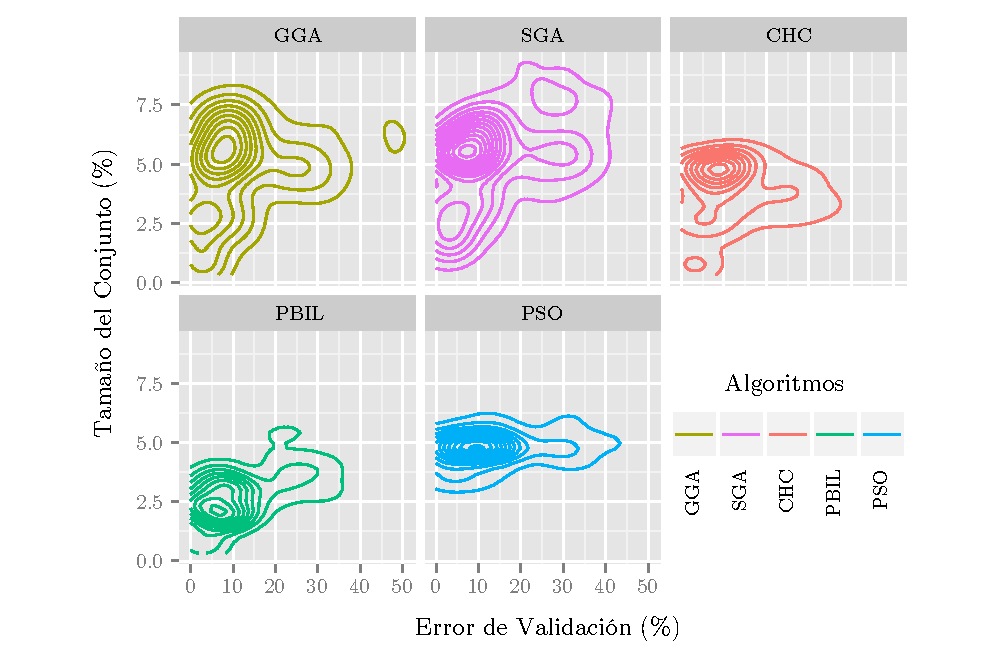
\includegraphics[width=\textwidth]{alg-density.pdf}
\caption[Distribución de los resultados de cada metaheurística]{Distribución de los resultados de cada metaheurística,\\en función del error de validación y el tamaño de las soluciones.}
\label{fig-alg-density}
\end{figure}

Esta gráfica confirma las conclusiones obtenidas a través de los datos presentados: PBIL muestra los mejores resultados en función de los objetivos del problema de SI. En comparación con las demás metaheurísticas, PBIL exhibe un comportamiento más estable, \emph{i.e.} la mayoría de sus soluciones presentan bajos porcentajes de error y tamaño. Al comparar estos datos con los de GGA, la gráfica de densidad muestra que los resultados de PBIL están mucho más concentrados en un área particular del plano, mientras que GGA presenta mayor variabilidad.

Para poder determinar con seguridad las posibles diferencias entre PBIL y el resto de las metaheurísticas, es necesario aplicar una prueba estadística. Se usa una prueba de rangos con signo de \emph{Wilcoxon} \cite{wilcoxon1945individual} (de cola inferior), con un nivel de significancia del $1\%$, para determinar si la mediana de la resultados de PBIL es menor que la de los resultados de las demás metaheurísticas en términos de error de validación o tamaño. A continuación se establecen las hipótesis de la prueba para este caso particular:

\begin{tabular}{l l}
$H_0$ & Los resultados de PBIL son mayores o iguales que los del algoritmo en cuestión.\\
$H_1$ & Los resultados de PBIL son menores que los del algoritmo en cuestión.\\
\end{tabular}

En función de estas hipótesis, en la tabla \ref{wilcox-res-pbil} se presenta el estadístico $W$ y el $p$-valor que permitirán rechazar o no la hipótesis nula $H_0$.

\begin{table}[h!]
\centering
\begin{tabular}{l c c c c}
\hline
\multirow{2}{*}{\textsc{Algoritmo}}
	& \multicolumn{2}{c}{\textsc{Error de Validación}}
	& \multicolumn{2}{c}{\textsc{Tamaño}} \\\cline{2-5}
 & $W$ & $p$-valor & $W$ & $p$-valor \\
\hline
\hline
GGA & 46 & $3.574 \times 10^{-1}$ &  1 & $1.221 \times 10^{-4}$ \\
SGA & 27 & $5.945 \times 10^{-2}$ &  0 & $6.104 \times 10^{-5}$ \\
CHC &  6 & $8.545 \times 10^{-4}$ & 14 & $6.714 \times 10^{-3}$ \\
PSO &  6 & $8.545 \times 10^{-4}$ &  0 & $6.104 \times 10^{-5}$ \\
\hline
\end{tabular}
\caption[Pruebas de \emph{Wilcoxon} entre PBIL y las demás metaheurísticas]{Estadístico $W$ y $p$-valor de pruebas de rangos con signo de \emph{Wilcoxon} para determinar si PBIL es mejor que el resto de las metaheurísticas, en función del error de validación y el tamaño de las soluciones encontradas.}
\label{wilcox-res-pbil}
\end{table}

Estos resultados permiten afirmar con un nivel de significancia del $1\%$, que PBIL exhibe mejores resultados que
\begin{inparaenum}[\itshape a\upshape)]
\item todas las metaheurísticas en términos de la reducción de los datos, y que
\item CHC y PSO en función al error de validación.
\end{inparaenum}
En resumidas cuentas, para encontrar soluciones al problema de SI, PBIL resulta la mejor opción en función de los objetivos del problema.

Sin embargo, debido a que el objetivo de estos algoritmos es que se apliquen sobre conjuntos de datos de tamaños grandes (mucho mayores a los conjuntos de datos evaluados en este estudio), la métrica del tiempo de ejecución es particularmente importante para evaluar las capacidades de las metaheurísticas para escalar a conjuntos mayores.

En este sentido, en la figura \ref{fig-tiempo} se grafica el aumento en tiempo de ejecución de las metaheurísticas en función del número de instancias de los 14 conjuntos de datos evaluados. Mientras que GGA, SGA, PBIL y PSO exhiben un aumento sustancial en el tiempo de ejecución, resulta evidente que CHC se ve menos afectado por el número de instancias que el resto de las metaheurísticas. Es destacable que CHC logre, en un tiempo significativamente menor, resultados competitivos en función del tamaño de las soluciones encontradas y manteniendo un error de validación aceptable. Esto hace de CHC el candidato perfecto para ser aplicado bajo conjuntos de datos con gran número de instancias.

\begin{figure}[h!]
\centering
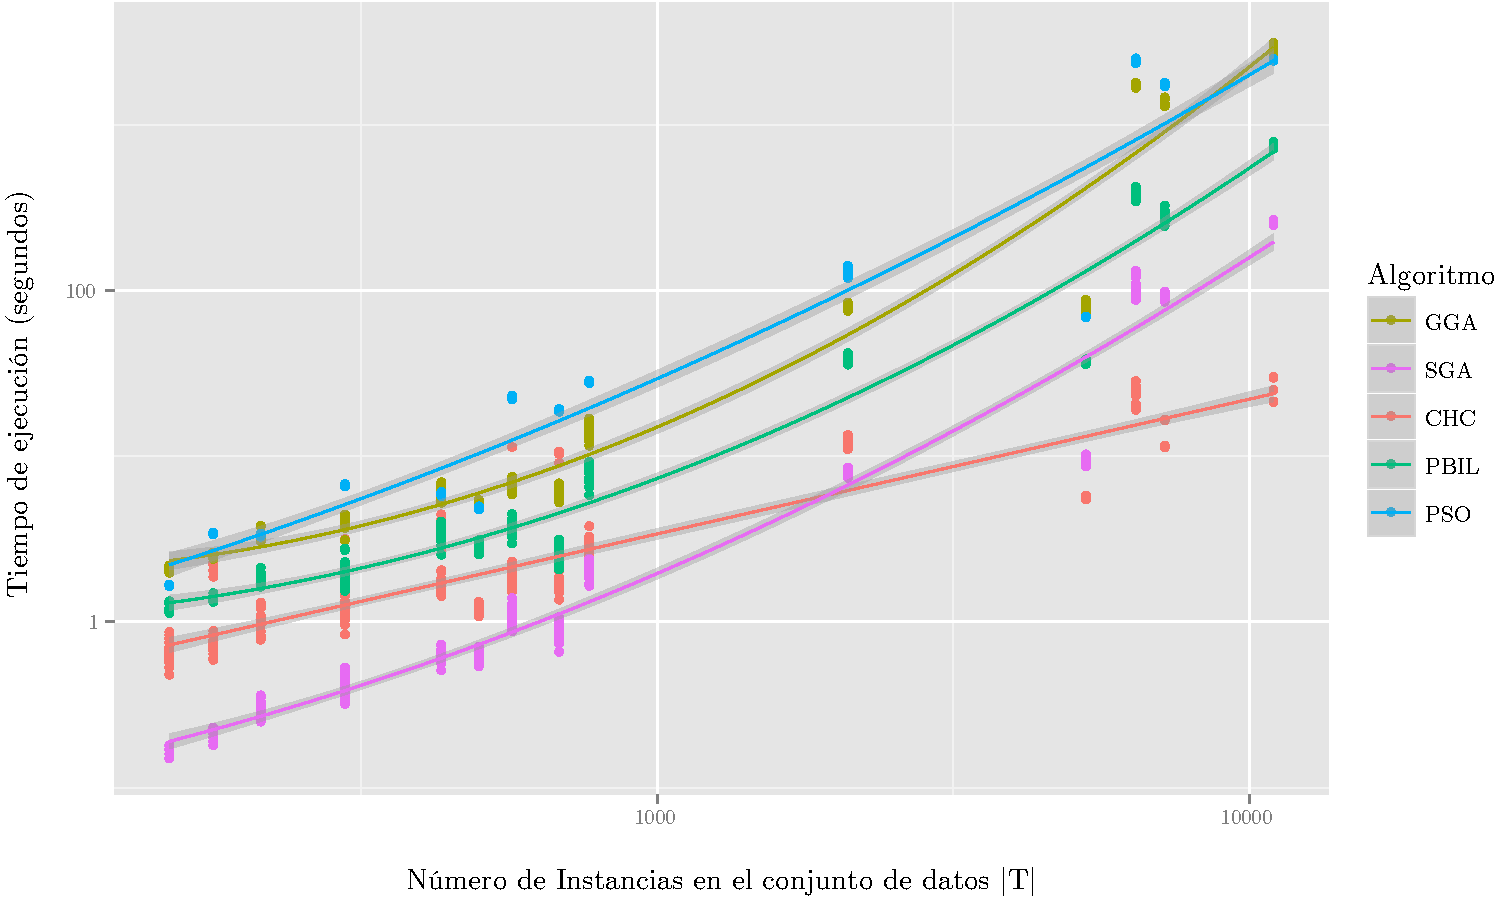
\includegraphics[width=0.9\textwidth]{tiempo.pdf}
\caption[Tiempo de ejecución de cada metaheurística]{Tiempo de ejecución reportado por cada metaheurística, usando el tiempo promedio en cada conjunto de datos, ordenándolos en función del número de instancias en cada conjunto de datos. Se usa escala logarítmica en ambos ejes.}
\label{fig-tiempo}
\end{figure}
